Debemos generar un directorio de p\'aginas que mapee con identity maping para el kernel un total de 1920 p\'aginas de 4 KB cada una, haciendo un total de 7,5 MB.
Para eso cargamos un Page Directory en la direcci\'on 0x27000, que contendr\'a 3 entradas que apuntan a 3 Directory Tables. Los primeros 2 Pages Tables son para las 1920 entradas que tenemos que mapear: 1024 para un Page Table, y 896 para el segundo.
Definimos un tercer Page Table para la tarea Idle.
El mapeo del directorio de p\'aginas ser\'a de esta forma:

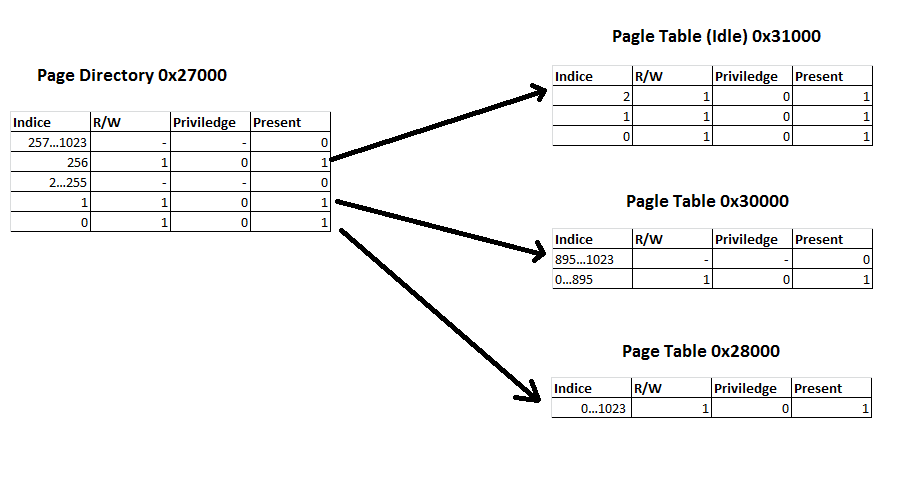
\includegraphics[scale=0.6]{imagenes/identity_mapping_kernel.png}


Luego de armar el directorio de p\'aginas podemos habilitar la paginaci\'on. Para esto debemos prender el bit mas significativo del registro CRO:\\
mov eax, [TASK\_PAG\_DIR]\\
mov cr3, eax\\
mov eax, cr0\\
or eax, 0x80000000\\
mov cr0, eax\\
